\chapter{Real World Testing}\label{ch:real.world.testing}

Several navigation methods and algorithms have been designed in Chapter \ref{ch:autonomous.navigation}. These algorithms have been evaluated on simulated environments and have provided, for the most part, good results. The last major step of this work is to test these functional algorithms on the real world, with a real drone.

This chapter presents and discusses the results of the different methods and algorithms adapted and tested in the real world. The different obtained results will help to discuss the feasibility of autonomous drone navigation in an indoor environment.

\section{Adaptation to real world}

The real drone used is a Tello EDU, presented in Chapter \ref{ch:controllers}. The controller of this drone, based on the high-level control interface presented in the same chapter, will be used.

The environment considered is the corridors the Montefiore Institute of the University of Liege. The representation of this environment presented in Section \ref{sec:05.montefiore.institute} will be used.

The various algorithms designed on the basis of the generic algorithm \ref{alg:06.generic.navigation.algorithm} will also be used without code modification. Their architecture, composed of several modules (see Section \ref{sec:06.architecture}), is still valid for the real drone. The only real modifications concern the methods \textsc{\textcolor{blue}{align}} and \textsc{\textcolor{blue}{analyze}}: the various modules created will be evaluated on real data in order to judge which modules could be used in practice or not.

\section{Alignment}

In order to align the drone on a straight trajectory when navigating in a corridor, two modules, working with the vanishing point, have been realized and tested on simulated environments: the \texttt{VPClassic} module detecting the vanishing point based on line detection and the \texttt{VPDeepLearning} module working with a Deep Learning model. Both modules were evaluated on real data.

\subsection{Line detection}

Two methods working with line detection had been evaluated previously: \texttt{VPClassic} and \texttt{VPEdgelets}. For its good results and its speed, the \texttt{VPClassic} method was retained.

The latter, with some adjustments of the different parameters of the methods (Canny algorithm and Hough transform) was evaluated on the real world. For this, a series of $\num{60}$ images, varied in terms of the position of the vanishing point, was collected (by manually controlling the drone). These images were then annotated with their vanishing point in the same way as the images collected in the simulated environments. Some examples of the collected images are shown in Figure \ref{fig:07.vanishing.point.evaluation.examples}.

\begin{figure}[H]
    \centering
    \begin{subfigure}{0.32\textwidth}
        \centering
        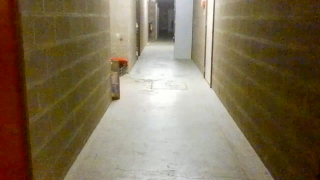
\includegraphics[width=\textwidth]{resources/png/07/vanishing-point/evaluation/0.png}
    \end{subfigure}
    \hfill
    \begin{subfigure}{0.32\textwidth}
        \centering
        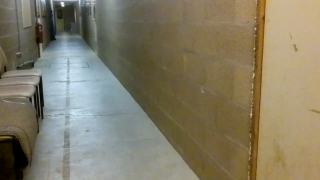
\includegraphics[width=\textwidth]{resources/png/07/vanishing-point/evaluation/1.png}
    \end{subfigure}
    \hfill
    \begin{subfigure}{0.32\textwidth}
        \centering
        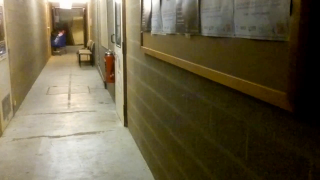
\includegraphics[width=\textwidth]{resources/png/07/vanishing-point/evaluation/2.png}
    \end{subfigure}
    \caption{Examples of images (real world) collected for the evaluation of the \texttt{VPClassic} vanishing point detection method.}
    \label{fig:07.vanishing.point.evaluation.examples}
\end{figure}

The \texttt{VPClassic} method was evaluated on these images in the same way as the images of the simulated environments (see Section \ref{sec:06.line.detection}). The obtained results are as follows: $\num{36}$ vanishing points were correctly detected over the $\num{60}$ images. The mean processing time per image is $\SI{0.05}{\second}$.

These results show that, despite its speed, this method is no longer efficient on real-world images. Only a little more than half of the vanishing points were detected correctly, which is too few to guarantee a correct navigation of the drone. The main problem seems to be the detection of the lines in the image. An example of a poorly detected vanishing point is shown in Figure \ref{fig:07.vpclassic.example}.

\begin{figure}[t]
    \centering
    \begin{subfigure}{0.49\textwidth}
        \centering
        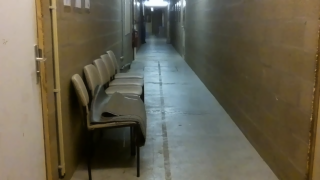
\includegraphics[width=\textwidth]{resources/png/07/vanishing-point/vpclassic/0.png}
        \caption{Bilateral filter}
        \vspace{0.5em}
    \end{subfigure}
    \hfill
    \begin{subfigure}{0.49\textwidth}
        \centering
        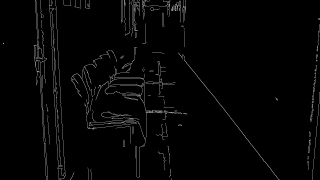
\includegraphics[width=\textwidth]{resources/png/07/vanishing-point/vpclassic/1.png}
        \caption{Canny filter}
        \vspace{0.5em}
    \end{subfigure}
    \begin{subfigure}{0.49\textwidth}
        \centering
        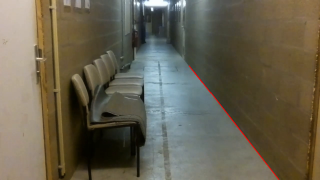
\includegraphics[width=\textwidth]{resources/png/07/vanishing-point/vpclassic/2.png}
        \caption{Filtered Hough transform}
    \end{subfigure}
    \hfill
    \begin{subfigure}{0.49\textwidth}
        \centering
        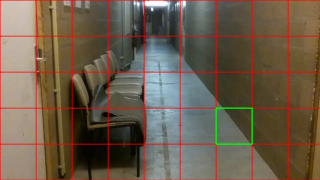
\includegraphics[width=\textwidth]{resources/png/07/vanishing-point/vpclassic/3.png}
        \caption{Extracted vanishing point}
    \end{subfigure}
    \caption{Example of results obtained via the \texttt{VPClassic} vanishing point detection method (image of real world).}
    \label{fig:07.vpclassic.example}
\end{figure}

In this example, it can be seen that the (static) obstacles on the left of the image obstruct the correct detection of the lines. In addition, the lines separating the ceiling from the walls are not visible. Therefore, only one line was correctly detected, which is not enough to determine the vanishing point.

Because of these degrading results and in order not to risk damaging the drone in case of bad detection, the \texttt{VPClassic} method was not retained for testing.

\subsubsection{Discussion}

It is interesting to try to understand why the results deteriorate so much when working on real world images.

The main difficulty seems to come from line detection. As mentioned in Chapter \ref{ch:autonomous.navigation}, line detection is a task that is far from trivial and difficult to generalize. Indeed, an algorithm that works very well under certain conditions may no longer work under other conditions.

The simulator images were of good quality, with good lighting conditions and clear distinction between floor, walls and ceiling. The real-world images, on the other hand, were sometimes blurred due to the movement of the drone, with sub-optimal lighting conditions and sometimes cluttered with static elements (\eg{} chairs). These conditions certainly degrade line detection.

\begin{note}
    It would certainly be possible to find improvements that would allow a better score on these images. However, it will remain difficult to design a very robust algorithm. For these reasons, and in view of the \texttt{VPDeepLearning} method presented in the next section, the \texttt{VPClassic} method has not been further developed in this work.
\end{note}

\subsection{Deep Learning}

A method working with a Deep Learning model has been evaluated on the simulated environments: \texttt{VPDeepLearning}. This method was also evaluated on real-world images.

For this, first, a data set of $\num{650}$ images (of size $\num{320} \times \num{180}$) was collected (by manually controlling the drone in the environment, see Section \ref{sec:06.image.classification}). Each of the images was annotated with its cell containing the vanishing point, in the same way as the images of the simulated environments. The data set was then separated into a training set ($\num{70}\%$ of the images) and a testing set ($\num{30}\%$ of the images).

The same model was kept: a modified version of the DenseNet-161 pre-trained model. The latter was trained in the same way and under the same conditions as for the images of the simulated environments.

The model was also evaluated using the same metrics. It obtained, on the testing set, a precision of $\num{0.92}$ and a recall of $\num{0.92}$. The mean processing time per image is $\SI{0.24}{\second}$. Although these results are slightly lower than those obtained on the simulated images, they are still very good. The problematic example via the line detection method was tested. The obtained results are shown in Figure \ref{fig:07.vpdeeplearning.example}.

\begin{figure}[H]
    \centering
    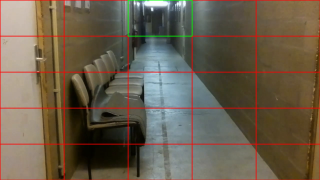
\includegraphics[width=0.6\textwidth]{resources/png/07/vanishing-point/vpdeeplearning/0.png}
    \caption{Example of a vanishing point detected via the \texttt{VPDeepLearning} method on a real world image.}
    \label{fig:07.vpdeeplearning.example}
\end{figure}

This example shows that the vanishing point has been correctly detected. In addition, the $\num{60}$ images used for the evaluation of the \texttt{VPClassic} method were also tested (these images are not from the training or the testing set used for the Deep Learning model). The model obtained a score of $\num{58}$ vanishing point correctly detected over $\num{60}$.

These results show that the \texttt{VPDeepLearning} method performs better than the \texttt{VPClassic} method on real world images. The latter was therefore retained for the alignment of the drone in the real world.

\subsubsection{Generalization}

The Deep Learning model involves the collection of images of the considered environment. This is not always possible, especially if the environment is not known in advance.

It is therefore interesting to study the extent to which a model trained on a simulator can be generalized to the real world. For this purpose, the DenseNet-161 model trained \emph{only} on the simulator images was evaluated on real world images. The model obtained, on the testing set, a precision of $\num{0.21}$ and a recall of $\num{0.13}$. These extremely poor results show that the model does not generalize at all to the real world. This can probably be explained by the fact that the simulator images are very different from the real world images and that the classification problem is complex (it is composed of $\num{25}$ different classes).

Inspired by the work of \textcite{anwar2020autonomous}, the DenseNet-161 model trained on the simulator images was taken up and trained, again, on the real-world images. However, only the last layers of the network (the extra layers added to the basic DenseNet-161 model, see Appendix \ref{ch:neural.networks.architectures}) were re-trained; the others remained fixed. With these conditions, the obtained results are as follows: a precision of $\num{0.68}$ and a recall of $\num{0.59}$. These results, although still poor, are clearly more encouraging. They show that a model pre-trained on a simulator and then trained on real images can provide usable results, but is still far from the performances of a model fully trained on real images.

Better results, and therefore better generalization, could perhaps be obtained via pre-training on more and varied images of simulated environments. The simulated environments could also try to be even closer to the real world. In the context of this work, having only two simulated environments, this aspect has been left for future work on the subject.

\section{Key points detection}

Several methods for key point detection based on drone images were created and evaluated on the simulated environments: \texttt{Vision} working with a Deep Learning model to perform image classification, \texttt{Depth} working with depth estimation and \texttt{Marker} working with marker detection and decoding.

These different methods were evaluated on real-world images.

\subsection{Image classification}

Image classification in the simulated environments was performed via the DenseNet-161 model. Each image was classified as either \enquote{key point} or \enquote{not key point}. This idea was retained and evaluated in the real world.

To do this, firstly, a data set of $\num{1570}$ images, including $\num{660}$ images of \enquote{key point} and $\num{910}$ images of \enquote{not key point}, was collected (by manually controlling the drone in the environment, see Section \ref{sec:06.image.classification}). The images were processed and annotated in the same way as the images of simulated environments. A sample is shown in Figure \ref{fig:07.classification.data.set.examples}.

\begin{figure}[H]
    \centering
    \begin{subfigure}{0.32\textwidth}
        \centering
        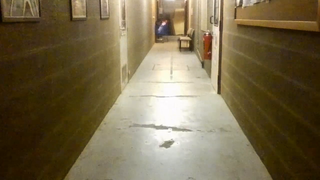
\includegraphics[width=\textwidth]{resources/png/07/classification/datasets/0.png}
        \vspace{0.5em}
    \end{subfigure}
    \hfill
    \begin{subfigure}{0.32\textwidth}
        \centering
        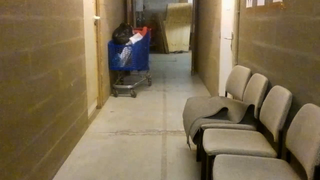
\includegraphics[width=\textwidth]{resources/png/07/classification/datasets/1.png}
        \vspace{0.5em}
    \end{subfigure}
    \hfill
    \begin{subfigure}{0.32\textwidth}
        \centering
        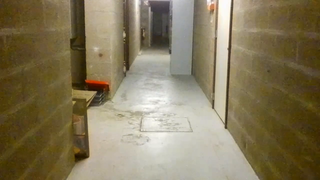
\includegraphics[width=\textwidth]{resources/png/07/classification/datasets/2.png}
        \vspace{0.5em}
    \end{subfigure}
    \begin{subfigure}{0.32\textwidth}
        \centering
        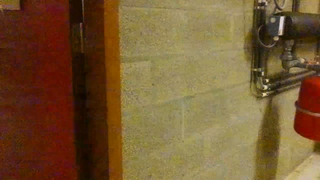
\includegraphics[width=\textwidth]{resources/png/07/classification/datasets/3.png}
    \end{subfigure}
    \hfill
    \begin{subfigure}{0.32\textwidth}
        \centering
        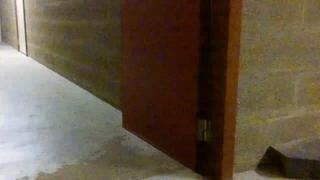
\includegraphics[width=\textwidth]{resources/png/07/classification/datasets/4.png}
    \end{subfigure}
    \hfill
    \begin{subfigure}{0.32\textwidth}
        \centering
        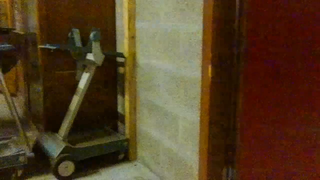
\includegraphics[width=\textwidth]{resources/png/07/classification/datasets/5.png}
    \end{subfigure}
    \caption{Example of images (real world) constituting the data sets for training the Deep Learning model. The first line contains images annotated as \enquote{not key point}. The second line contains images annotated as \enquote{key point}.}
    \label{fig:07.classification.data.set.examples}
\end{figure}

The data set was then separated into a training set ($\num{70}\%$ of the images) and a testing set ($\num{30}\%$ of the images).

The DensetNet-161 model was trained and evaluated under the exact same conditions as the images of the simulated environments. The obtained results, on the testing set, are the following: a precision of $\num{1}$ and a recall of $\num{0.99}$. The mean processing time per image is $\SI{0.25}{\second}$. These excellent results show that the model is perfectly capable of adapting to more complex images from the real world. The \texttt{Vision} module will therefore be retained to carry out the various tests.

\subsubsection{Generalization}

Again, it is interesting to test how well a model trained only on a simulated environment can generalize to the real world.

To do this, two versions of the DenseNet-161 model trained on the images of the simulated Indoor Staircase environment (since the real-world images contain staircases, only the Indoor Staircase environment was considered) were evaluated on the real-world images: one version trained on the images and another trained on the edges of the images. The results are presented in Table \ref{tab:07.classification.generalization.evaluation}.

\begin{table}[H]
    \centering
    \begin{tabular}{|l|l|c|c|}
        \hline
        \textbf{Training} & \textbf{Evaluation} & \textbf{Precision} & \textbf{Recall} \\ \hline
        Indoor Staircase & Real-world images & $\num{0.98}$ & $\num{0.51}$ \\ \hline
        Indoor Staircase (on edges) & Real-world images & $\num{0.98}$ & $\num{0.78}$ \\ \hline
    \end{tabular}
    \caption{Evaluation of the generalizability across (real and simulated) environments of the DenseNet-161 model for the image classification problem.}
    \label{tab:07.classification.generalization.evaluation}
\end{table}

These results, which are much more encouraging than those of the vanishing point, show that the model seems to generalize well to the real world. This can be explained by the fact that the classification problem only contains two different classes and that these classes are easily distinguishable (the model can easily makes a clear difference between a corridor and a wall).

Similar to the tests performed on simulated environments, training on image edges gives better results for the generalization of the model. These results are very interesting because they show that it could be possible to teach a drone to fly in an environment that is totally unknown to it on the basis of training carried out only on a simulator. This model, trained on the simulator's image edges, will be kept for flight tests and will be called \texttt{VisionGen}.

\subsection{Depth estimation}

Depth estimation via a pre-trained model was the second method tested on the simulated environments for key point detection (\texttt{Depth} module).

The chosen pre-trained model, MiDaS, was tested on real-world images under the same conditions as the images in the simulated environments. Some examples of the obtained results are shown in Figure \ref{fig:07.depth.results.examples}.

\begin{figure}[H]
    \centering
    \begin{subfigure}{0.32\textwidth}
        \centering
        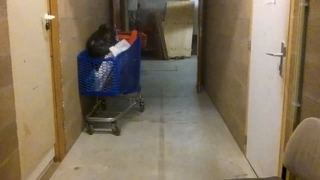
\includegraphics[width=\textwidth]{resources/png/07/depth/original/0.png}
        \vspace{0.5em}
    \end{subfigure}
    \hfill
    \begin{subfigure}{0.32\textwidth}
        \centering
        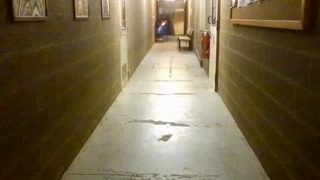
\includegraphics[width=\textwidth]{resources/png/07/depth/original/1.png}
        \vspace{0.5em}
    \end{subfigure}
    \hfill
    \begin{subfigure}{0.32\textwidth}
        \centering
        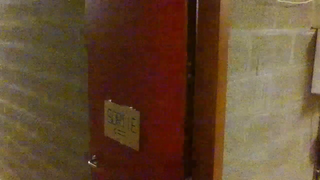
\includegraphics[width=\textwidth]{resources/png/07/depth/original/2.png}
        \vspace{0.5em}
    \end{subfigure}
    \begin{subfigure}{0.32\textwidth}
        \centering
        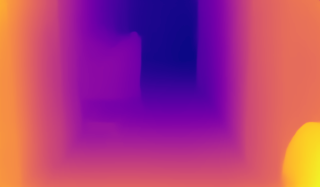
\includegraphics[width=\textwidth]{resources/png/07/depth/results/0.png}
    \end{subfigure}
    \hfill
    \begin{subfigure}{0.32\textwidth}
        \centering
        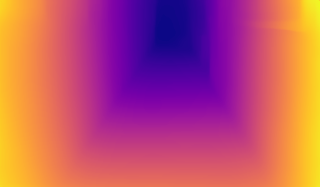
\includegraphics[width=\textwidth]{resources/png/07/depth/results/1.png}
    \end{subfigure}
    \hfill
    \begin{subfigure}{0.32\textwidth}
        \centering
        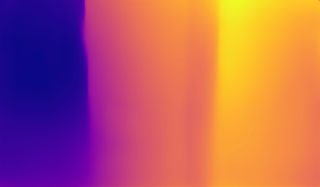
\includegraphics[width=\textwidth]{resources/png/07/depth/results/2.png}
    \end{subfigure}
    \caption{Examples of obtained results with the MiDaS pre-trained model. The first row contains the original images (real world). The second row contains the corresponding inferred relative depth maps.}
    \label{fig:07.depth.results.examples}
\end{figure}

The obtained results are, as for the images of the simulated environments, quite convincing. Moreover, the key point detection procedure has been evaluated on the testing set (real images) used for the DenseNet-161 model, as it was in the Chapter \ref{ch:autonomous.navigation}: a precision of $\num{0.78}$ and a recall of $\num{0.74}$ have been obtained.

The \texttt{Depth} module was therefore retained for the flight tests.

\subsection{Markers}

The use of markers to be detected and decoded was the third method used for key point detection (\texttt{Marker} module).

For their efficiency and speed of detection and decoding, only the ArUco markers were retained. The latter were evaluated on real-world images in the same way as the images of the simulated environments. For this purpose, a series of $\num{100}$ images containing an ArUco marker, with as many different angles of view as possible, was collected. Some examples of the images are shown in Figure \ref{fig:07.markers.aruco.examples}.

\begin{figure}[H]
    \centering
    \begin{subfigure}{0.32\textwidth}
        \centering
        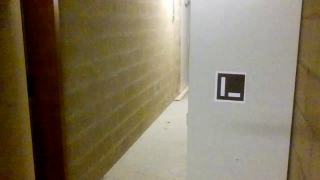
\includegraphics[width=\textwidth]{resources/png/07/markers/aruco/0.png}
    \end{subfigure}
    \hfill
    \begin{subfigure}{0.32\textwidth}
        \centering
        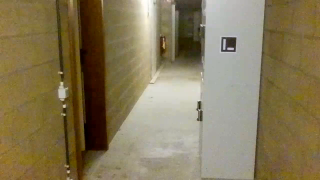
\includegraphics[width=\textwidth]{resources/png/07/markers/aruco/1.png}
    \end{subfigure}
    \hfill
    \begin{subfigure}{0.32\textwidth}
        \centering
        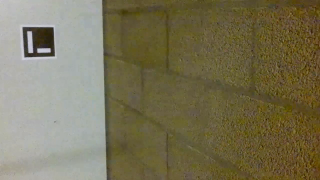
\includegraphics[width=\textwidth]{resources/png/07/markers/aruco/2.png}
    \end{subfigure}
    \caption{Examples of (real-world) images collected for the evaluation of the ArUco marker detection and decoding method.}
    \label{fig:07.markers.aruco.examples}
\end{figure}

The obtained results are as follows: $\num{100}$ markers were detected and decoded correctly over the $\num{100}$ images. The mean processing time per image is $\SI{0.006}{\second}$.

Not surprisingly, the obtained results are, as for the simulated environments, excellent. For this reason, the \texttt{Marker} module was retained for the flight tests.

\section{Autonomous navigation algorithms}

Several autonomous navigation algorithms have been created and evaluated on the simulated environments: \texttt{NavVision} using the \texttt{Vision} module, \texttt{NavDepth} using the \texttt{Depth} module and \texttt{NavMarker} using the \texttt{Marker} module.

These different algorithms have been tested in the real world. The different modules have been adapted to the real world, as explained above. A new navigation algorithm was also created based on the module \texttt{VisionGen}: \texttt{NavVisionGen}. The latter is exactly the same as the \texttt{NavVision} algorithm but works with the model trained on the simulator (\texttt{VisionGen}) in order to experiment with Transfer Learning.

The different robust algorithms, presented in Section \ref{sec:06.robustness}, have also been evaluated. As mentioned in this same section, the verification based on the environment (\texttt{+ Env}) has not been kept.

Finally, each algorithm uses the \texttt{VPDeepLearning} module for the alignment of the drone.

Two trajectories were defined, in the Montefiore Institute, to evaluate the different algorithms. These are shown in Figure \ref{fig:07.evaluation.trajectories}.

\begin{figure}[H]
    \centering
    \begin{subfigure}{0.49\textwidth}
        \centering
        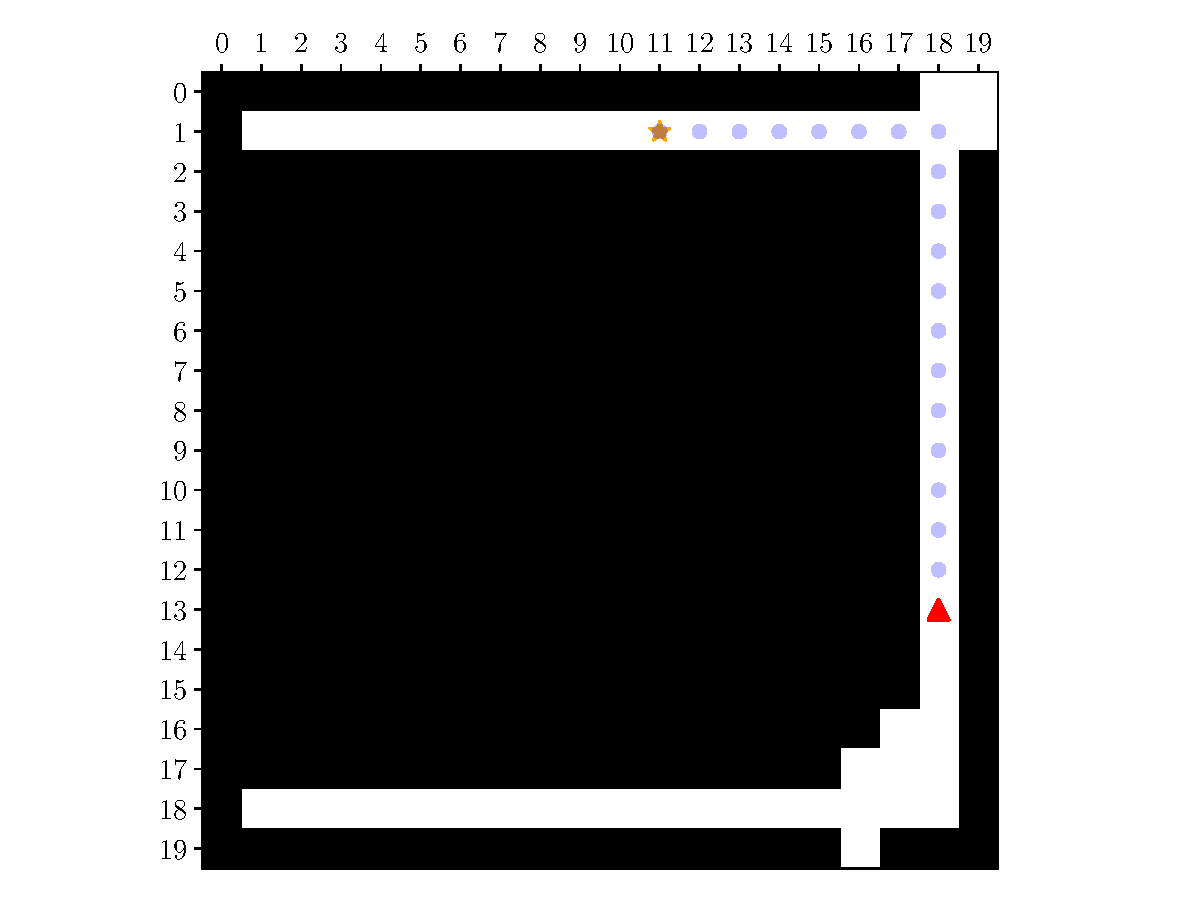
\includegraphics[width=\textwidth]{resources/pdf/07/evaluation/0.pdf}
        \caption{Trajectory 1}
    \end{subfigure}
    \hfill
    \begin{subfigure}{0.49\textwidth}
        \centering
        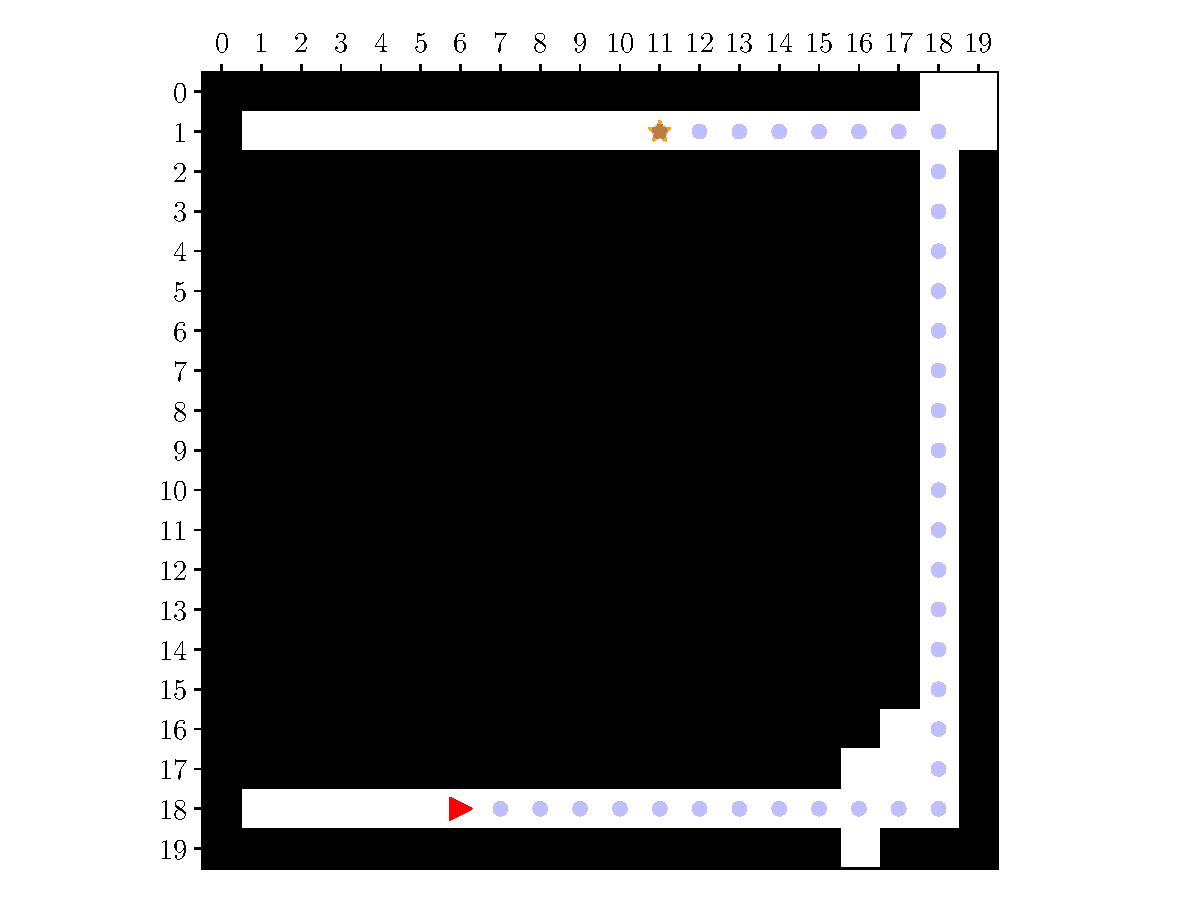
\includegraphics[width=\textwidth]{resources/pdf/07/evaluation/1.pdf}
        \caption{Trajectory 2}
    \end{subfigure}
    \caption{Trajectories used for the evaluation of the different navigation algorithms (real world). The starting point of the drone, as well as its orientation, is represented by a red arrow. The objective to be reached is represented by a yellow star. The path to follow is represented by blue dots.}
    \label{fig:07.evaluation.trajectories}
\end{figure}

The first is a simple trajectory containing only one turn. The second is a more difficult one containing two turns. The first turn of this difficult path is actually almost a crossroads as it is an open space with staircases and several recesses in the walls.

Each algorithm was evaluated in the same way as for the simulated environments. However, due to technical constraints with the battery autonomy of the drone, each trajectory was only tested $\num{10}$ times. The obtained results are presented in Table \ref{tab:07.evaluation.results}.

\begin{table}[t]
    \centering
    \begin{tabular}{|l|c|c|}
        \hline
        \textbf{Algorithm} & \textbf{Trajectory} & \textbf{Full-Flight Ratio} (FFR) \\ \hline
        \hline
        \multirow{2}{*}{\texttt{NavVision}} & 1 & \num{0.8} \\ \cline{2-3}
        & 2 & \num{0.7} \\ \hline
        \multirow{2}{*}{\texttt{NavVisionGen}} & 1 & \num{0.7} \\ \cline{2-3}
        & 2 & \num{0.6} \\ \hline
        \multirow{2}{*}{\texttt{NavDepth}} & 1 & \num{0.4} \\ \cline{2-3}
        & 2 & \num{0.2} \\ \hline
        \multirow{2}{*}{\texttt{NavMarker}} & 1 & \num{0.9} \\ \cline{2-3}
        & 2 & \num{0.9} \\ \hline
        \multirow{2}{*}{\texttt{NavVision + Depth}} & 1 & \num{0.9} \\ \cline{2-3}
        & 2 & \num{0.7} \\ \hline
        \multirow{2}{*}{\texttt{NavVision + Marker}} & 1 & \num{1} \\ \cline{2-3}
        & 2 & \num{0.9} \\ \hline
    \end{tabular}
    \caption{Results of the evaluation of different navigation algorithms on two pre-defined trajectories (real world).}
    \label{tab:07.evaluation.results}
\end{table}

A flight demonstration on the trajectory 1 using the \texttt{NavVision} algorithm is available via the following link: \url{https://youtu.be/-GHyQnuI1Gk}.

\subsection{Discussion}

The obtained results allow several observations.

Firstly, in general, the results show that the drone is able to navigate from a starting point to an objective autonomously in a real indoor environment, based solely on the monocular images of its RGB front camera.

Secondly, we observe that, once again, the algorithms working with markers provide the best results. This is not a surprise since markers are detected very efficiently and allow a (more or less accurate) estimation of the distance of the drone to the key point. However, as already mentioned, markers can only be used if the environment is accessible for pre-processing.

Thirdly, the algorithm \texttt{NavVision} provides good results. In the vast majority of trials, the drone succeeded in reaching its objective. In addition, the algorithm \texttt{NavVisionGen} also seems to provide correct results. Although a little less good, they nevertheless show that a model trained on simulator can be used in the real world to navigate a drone.

Fourthly, we observe that the \texttt{NavDepth} algorithm does not give good results. Having a too rough estimation of the environment (especially since it is a pre-trained model that has not been fine tuned on the considered environment), the drone tends to make too many errors in its detections.

Finally, we observe that robust algorithms provide slightly better results than non-robust algorithms.

In view of the obtained results, it is possible to fly a drone autonomously in an indoor environment. Markers are, for the moment, the most efficient solution. However, they cannot be used when the environment cannot be processed in advance. In this case, the algorithm \texttt{NavVision} can be used. The latter has proved, in all the tests carried out, to be really efficient and quite simple for the detection of key points in the environment. The good results obtained with the \texttt{NavVisionGen} algorithm are very promising and show that Transfer Learning can be a feasible solution for creating drones capable of navigating in environments that are totally unknown to them.

\section{Advanced navigation}

In order to further develop the results, the management of battery stations in the environment and the passage of staircases were tested in simulated environments. These were also tested in the real world.

\subsection{Battery station}

In order to test the drone's ability to plan a path to a battery station and land there, a fictitious battery station was imagined at the Montefiore Institute. This can be located by an ArUco marker placed directly above it on the wall.

Based on its representation of the environment and the position of this known charging station, a simple path was planned (Figure \ref{fig:07.advanced.battery.path}).

\begin{figure}[H]
    \centering
    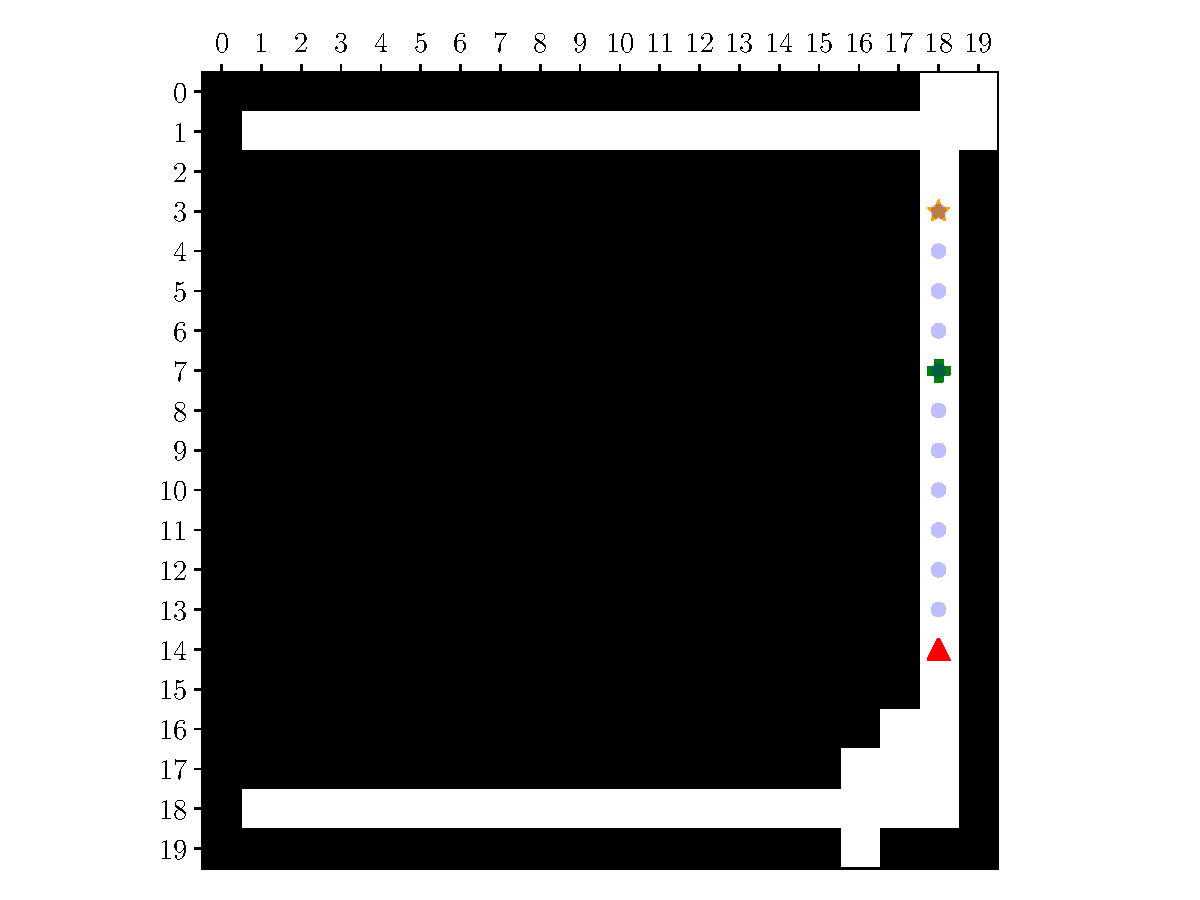
\includegraphics[width=0.55\textwidth]{resources/pdf/07/battery/path.pdf}
    \caption{Example of a path planned by the drone and passing through a battery station (green cross) in the real-world environment.}
    \label{fig:07.advanced.battery.path}
\end{figure}

Similar to the tests performed in the simulated environment, the drone uses the \texttt{NavVision + Depth} algorithm to move and reach its objectives. When the drone reaches the battery station, it performs a $\SI{360}{\degree}$ rotation to try to locate the ArUco marker. When the ArUco marker is located, the drone uses the \texttt{Marker} module to align itself and land on the battery station. It stops for a few seconds and then heads back to its final destination.

A small demonstration is available in a video via the following link: \url{https://youtu.be/M0i27bwo5Z8}.

This algorithm was evaluated $\num{10}$ times in the same way as the one used for the simulated environment. The results obtained are as follows: the drone successfully completed $\num{9}$ of the $\num{10}$ trials. This very good result shows that it is possible quite easily, even in a real environment, to include charging stations in the environment, which is a real advantage for drones with low autonomy.

\subsection{Staircase}

Different methods for staircase crossing were created and tested on the simulated environments: a naive method, a method based on depth estimation and a method using markers. As the depth estimation method did not provide satisfactory results in the simulated environment, it was not tested in the real one.

To test the different methods, a simple path through a staircase in Montefiore was defined. This path, shown in Figure \ref{fig:07.advanced.staircase.path}, presents no other difficulties apart from the staircases.

\begin{figure}[H]
    \centering
    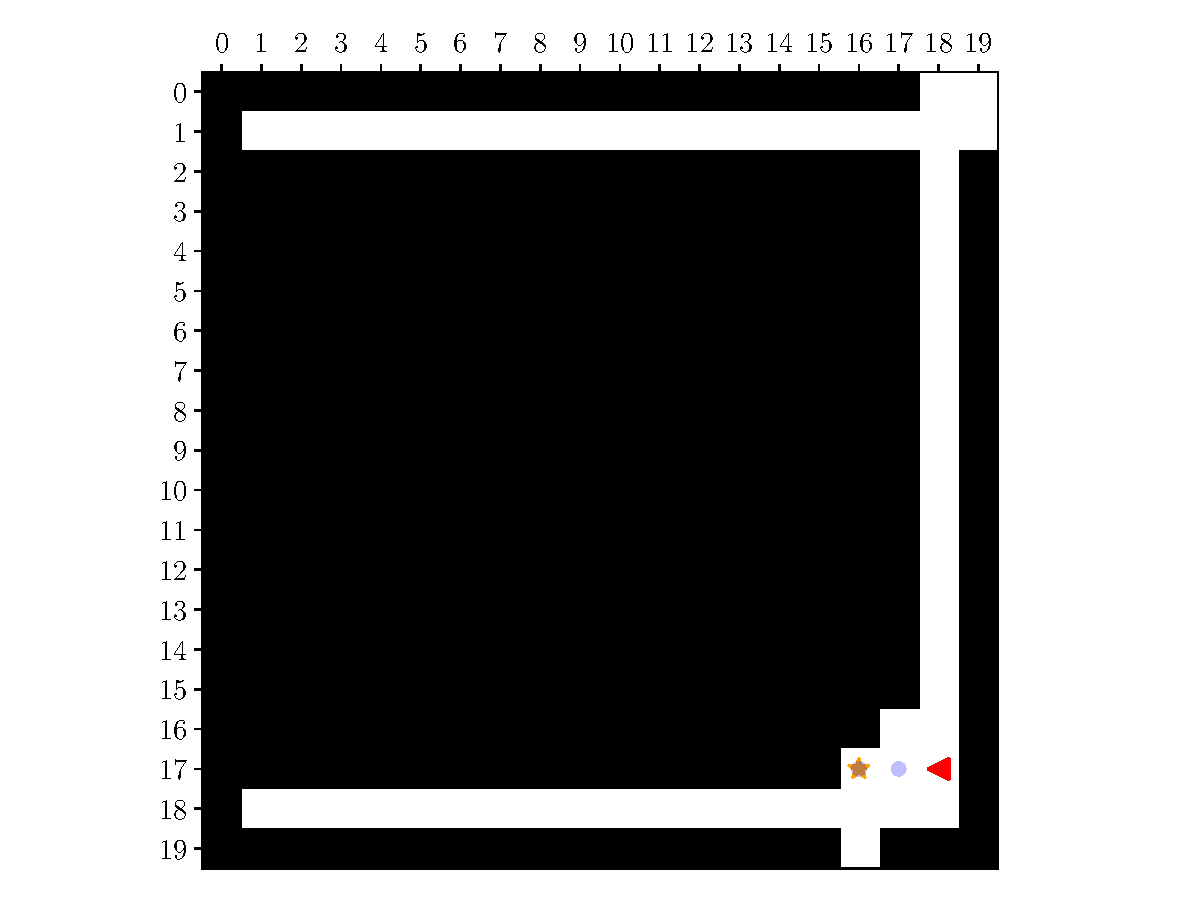
\includegraphics[width=0.55\textwidth]{resources/pdf/07/staircase/path.pdf}
    \caption{Example of a path planned by the drone and passing through a staircase in the real-world environment.}
    \label{fig:07.advanced.staircase.path}
\end{figure}

It should be noted that this staircase, in the real world, turns in several places before reaching the top floor. Since the algorithms are not designed for this type of staircase, the drone is stopped when it reaches the first landing and the passage is considered successful.

Identical to the simulated environment tests, the \texttt{NavVision + Depth} algorithm was used. The trajectory was tested $\num{10}$ times. The obtained results are shown in Table \ref{tab:07.evaluation.staircase.results}.

\begin{table}[H]
    \centering
    \begin{tabular}{|l|c|}
        \hline
        \textbf{Algorithm} & \textbf{Full-Flight Ratio} (FFR) \\ \hline
        \hline
        \texttt{NavVision + Depth + StaircaseNaive} & \num{0.8} \\ \hline
        \texttt{NavVision + Depth + StaircaseMarker} & \num{0.9} \\ \hline
    \end{tabular}
    \caption{Results of the evaluation of different staircase crossing methods on a pre-defined trajectory (real-world).}
    \label{tab:07.evaluation.staircase.results}
\end{table}

A small demonstration, using \texttt{StaircaseMarker}, is available via the following link: \url{https://youtu.be/BaQX4N4wwAM}.

It can be seen that, as with the simulated environment tests, both methods appear to be effective for staircase passage. However, as explained above, the naive method cannot be generalized to all types of staircases and may not work in all types of environment. In addition, it is not robust. On the contrary, the method using markers can be adapted to several types of staircases (differing by their slope) and is more robust since it allows the drone to know its distance to the staircases.

These fairly simple tests obviously do not allow for a complete passage of difficult staircases but are nevertheless very encouraging and pave the way for future work on complex staircases.

\section{Summary}

In this chapter, the different methods tested on simulator have been adapted and evaluated in the real world.

First, the modules \texttt{VPClassic} and \texttt{VPDeepLearning} allowing the alignment of the drone via the calculation of the vanishing point of an image were tested. The module \texttt{VPClassic} gives much less good results than on simulator. The module \texttt{VPDeepLearning} still gives, on the other hand, good results.

The modules \texttt{NavVision}, \texttt{NavDepth} and \texttt{NavMarker} were also tested. The obtained results on the real world still seem good. The generalization of the model used for the module \texttt{NavVision} has also been tested. For that, the model was trained on simulator and directly used on the real world. The obtained results show that this solution, despite slightly lower scores, is promising.

Based on the modules providing good results, different navigation algorithms have been tested. The algorithm working with depth estimation does not provide good results. The other algorithms, working with image classification and marker detection, provide good results. The robust algorithms have also been tested and, once again, improve the obtained results.

Finally, the staircase passage and battery stations have been tested. The naive method and the method using markers allowed the drone to successfully pass staircases. The battery stations, on the other hand, were successfully detected using ArUco markers.
